\chapter{Deep Learning for 21cm Observations}
\label{chapter:hera_ml}

Modern cosmological theory is capable of predicting the statistical features of many aspects of the observable Universe, using either theoretical calculations \citep[e.g.][]{Bond.91, Sheth.99} or sophisticated numerical simulations \citep[e.g.][]{Lewis.00, Vogelsberger.14}. These theories may be tested by making observations of various large-scale fields, in surveys spanning large cosmological volumes in space and time. The ultimate goal of measurements is extract from the data some parameters which are believed to describe the underlying processes, and to relate these parameters to a theoretical understanding of the physics at work. In some cases -- most conspicuously the primordial CMB -- the statistics of the fields are Gaussian, and are completely described by the two-point correlation function, or its Fourier conjugate, the power spectrum \citep[e.g.][for a review]{Liddle.00}.

A field described only by Gaussian statistics practically does not exist in cosmology beyond the CMB. For nearly every other scenario involving the non-linear interactions of gravity, radiation, and fluid mechanics, the resultant fields are non-Gaussian. Within the non-Gaussianity of these fields is encoded additional valuable information about the astrophysical processes at work, and can also serve as a cross-validation of two-point statistics of the same field \citep{Alvarez.16, Majumdar.17}. The specific details of the non-Gaussianity are not usually straightforwardly obtained from the theory, and thus devising appropriate higher-order statistics to efficiently probe the non-Gaussian information is in general a difficult problem. 

By analyzing a field using power spectra, one explicitly neglects all non-Gaussian information. In Chapter~\ref{chapter:ksz_21cm}, we presented higher-order correlation functions that are sensitive to non-Gaussian information in Fourier space. In the case of 21\,cm emission, working in Fourier space provides a natural and relatively simple way to avoid foreground contamination. Another solution could be to search for non-Gaussian information in image space, assuming some future development that could overcome the foreground challenge \citep[e.g.][]{Shaw.14, Shaw.15, Zhu.16, Patil.17}, or that we may operate on wedge-filtered image fields in a physically meaningful way \citep{Beardsley.15}. Staying in image space allows us to retain the non-Gaussian information in our data.

\section{Neural Networks}

A potential solution for parameter extraction is available due to advances in computation, allowing us to generate large numbers of numerical simulations which are realizations that capture the relevant physics of an astrophysical process \citep[e.g.][]{Mesinger.11}, and the development of deep learning algorithms which can be ``trained'' to recognize patterns in data \citep[e.g.][]{Hinton.06, Hinton.12}.

Convolutional Neural Networks \citep[CNNs; e.g.][]{Lecun.95} have proven exceptionally useful for extracting non-Gaussian information from images in order to classify or extract information from their contents to a very high accuracy \citep[e.g.][]{imagenet.12}. There are many, many explanations of the inner calculus of neural networks, and the intention of this chapter is not a comprehensive review of that field. For the purposes of this chapter, a few concepts must be mentioned:

\begin{itemize}
\item Convolutional Neural Networks are systems of 1, 2 or 3-dimensional matrices that are used as convolutional kernels on an input image. An image is propagated forward through the network via consecutive convolutions by these kernels. Each kernel entry (i.e. pixel) is known as a `weight' $w$.

\item The desired output of a `training set', for example, the contents of an image, is given as a vector which the total of all the convolutions must reproduce.

\item Inevitably, if the convolutional kernels are initially randomly generated, the output vector will not contain the desired quantities. A `cost function' is a metric that specifies how `wrong' an output is. This could be the mean squared error, for example.

\item Neural networks `learn' through a process called `backpropagation'. Based on the cost function, a chain rule can be applied backwards along the network for each input, updating the values of the weights by some fraction of the user-specified `learning rate' \citep{Rumelhart.86}.

\item Associated with each weight is an `activation function', $a(x)$. The value of $a(w*x)$ (the output of the activation function given the convolved input) is actually what is handed to the next convolutional kernel along the network. Activation functions can be non-linear, allowing neural networks to learn complex decision boundaries.

\item In order to down-sample the data to a more manageable size, `pooling layers' are often implemented. These extract a moving statistic such as the moving average or maximum in a given region of the image.

\item CNNs often end with a `fully connected' or `dense' layer. These are multi-layer perceptrons \citep[e.g.][]{Rosenblatt.61} that propagate the value s of $a(wx)$ -- that is, no convolution is applied, and each layer is 1-dimensional.

\item After training on some subset of the total data (which may be done several times over), a neural network can be `tested' by forward-propagating new images, not used in training, and not backpropapating. Testing can also be implemented after some subsample of the training data has been propagated -- i.e., as the network is in the middle of training -- often called `validation'.
\end{itemize}

With this primer in mind, we will present two uses of CNNs for understanding simulated realizations of reionization: classifying the main causes (galaxies or active galactic nuclei) of reionization \citep{Hassan.18}, and regressing upon a physical parameter of interest.

\section{Classifying reionization models}

The 21\,cm power spectrum is a powerful tool for quantifying the relative clustering of large and small scaled ionized regions \citep{Hassan.17}. However, the topology of the regions themselves can provide information on the dominant mechanism of their formation. We considered two scenarios: one in which only galaxies, and the other in which only active galactic nuclei (AGN), provided ionizing photons. 

We used {\sc simfast21} \citep{Santos.10, Hassan.17.1} to generate a dark matter density field, evolve it into the non-linear regime using the Zel'dovich approximation. Dark matter halos were generated using the excursion set formalism \citep{Bond.91}. Either galaxies or AGN were placed in halos, with populations following the parametrization of \cite{Hassan.16}. Ionized regions are ``painted on top of'' the dark matter halos according to parametrizations from high-resolution radiative transfer simulations and large-volume hydrodynamic simulations (see \cite{Hassan.16, Hassan.18}). An example of a galaxy-dominated and AGN-dominated reionization field is shown in Figure~\ref{fig:hassan-fields}. For this study, we focused on the field at redshift $z=8$. Galaxies produce more, small, ionized regions, whereas AGN produce larger more spherical ones. This is due to the strong clustering AGN and their harder X-ray spectrum.

\begin{figure}
\centering
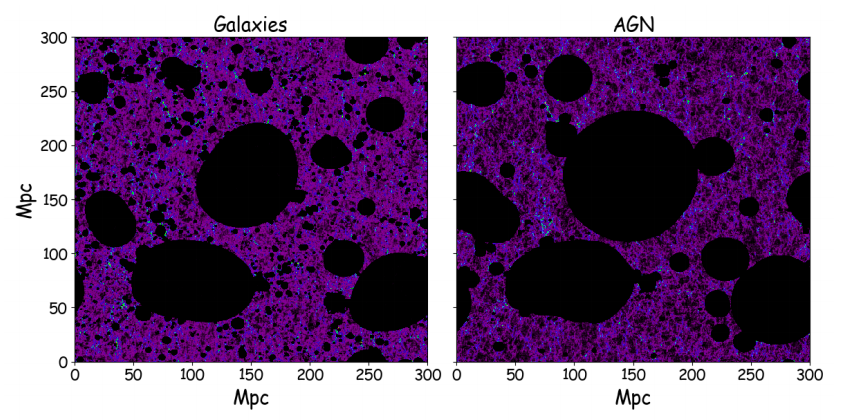
\includegraphics[width=0.8\textwidth]{chapters/hera_ml/figures/hassan-field.png}
\caption[21\,cm brightness temperature fields for Galaxy-Only and AGN-only models.]{21\,cm brightness temperature fields (in arbitrary units) for Galaxy-Only (left) and AGN-only (right) models. Figure from \cite{Hassan.18}.}
\label{fig:hassan-fields}
\end{figure}

We used {\tt Tensorflow} \citep{tensorflow} to build a classifying CNN with 2 layers of 2-dimensional convolutional kernels interleaved with two maximum-pooling layers, a single dense layer, and an output layer. The convolutional and dense layers used the ReLU activation function, which is defined as

\begin{equation}
{\rm ReLU}(x) = 
\begin{cases} 
      0 & x < 0 \\
      x & x >0 
\end{cases}
\end{equation}

\begin{figure}
\centering
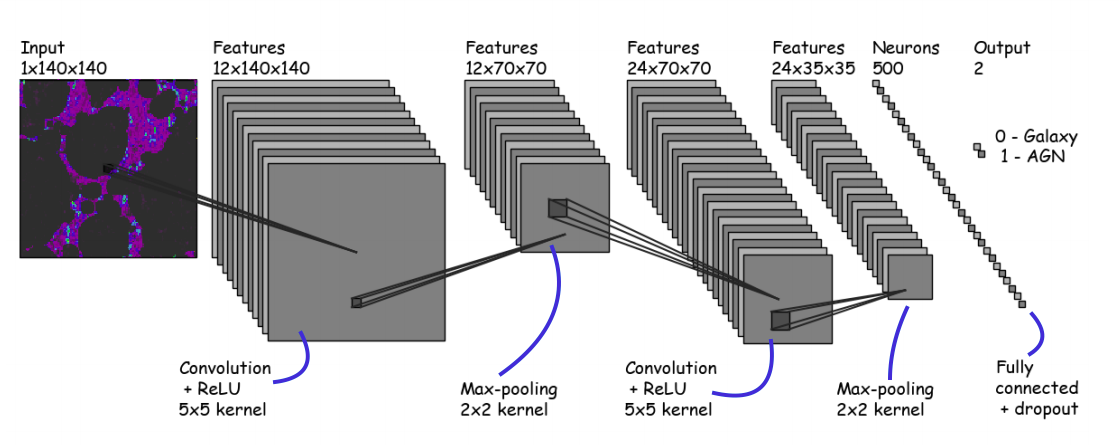
\includegraphics[width=0.8\textwidth]{chapters/hera_ml/figures/hassan-cnn.png}
\caption[The classification CNN used in this study.]{The classification CNN used in this study. Figure taken from \cite{Hassan.18}.}
\label{fig:hassan-cnn}
\end{figure}

The network is shown in Figure~\ref{fig:hassan-cnn}. To train it, we used $\sim 1000$ images of $z=8$ realizations. Each image was a $140\times140$ greyscale image of 21\,cm brightness temperature, with a simulation box size of 75\,Mpc. Each image came from a separate simulation, which varied the photon escape fraction, X-ray spectrum of the ionizing sources and the ionizing efficiency of those sources. The testing set was $\sim 100$ additional images. To prevent over-fitting, only a random set of 75\% of neurons were used during each forward propagation (a method known as `dropout'). The logistic cross-entropy function was used as the cost function.

Using the {\sc 21cmSense} package \citep{Pober.14}, we could simulate the expected thermal noise of a foreground-decontaminated image cube for LOFAR, HERA-331 and SKA-Low (see Chapter~\ref{chapter:instruments}). Adding this noise to each image allowed us to make predictions of the accuracy of such a tool for predicting ionization models for actual data.

The results of training and validation are shown in Figure~\ref{fig:hassan-results}. During training, the HERA and SKA fields quickly become $>99\%$ accurately classified. Systematic gaps between training and validation data for HERA suggests that an additional linear bias parameter may be useful for future networks. While the LOFAR classification eventually reaches high accuracy during training, validation shows that the network is strongly overfitting in this case -- suggesting that LOFAR will not be able to produce data in which the galaxy and AGN contributions to reionization. This result is substantiated by power spectrum studies by \cite{Hassan.17}.

\begin{figure}
\centering
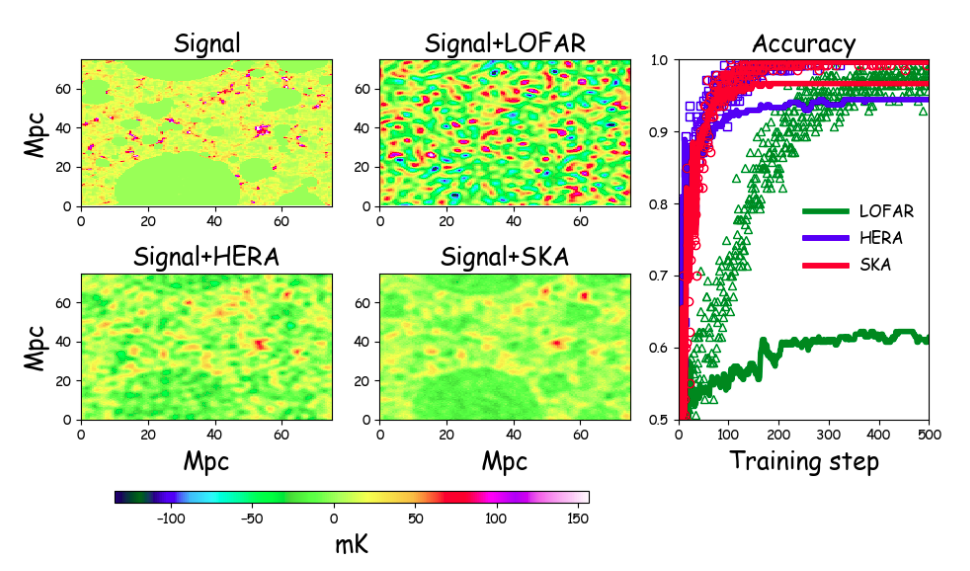
\includegraphics[width=0.8\textwidth]{chapters/hera_ml/figures/hassan-results.png}
\caption[Training data and results of the classifier.]{Training data and results of the classifier. On the left, an example 21\,cm brightness temperature field from the training set, with different thermal noise instances according to instrument designs. On the right, the accuracy of training (open symbols) and testing (sold lines) for the three different instruments considered. Figure taken from \cite{Hassan.18}.}
\label{fig:hassan-results}
\end{figure}

We can inspect the effect that kernels of a given layer have on an input image to gain some interpretation of what the network regards as `important' for the classification. An example of such an inspection is shown in Figure~\ref{fig:CNN_kernel_images}, which shows a single (galaxy-dominated) training image propagated through the trained kernels of the first convolutional layer. Some form of edge detection emphasizing the small, high-temperature regions of the map has been learned by the kernels. A comprehensive understanding of the relationship between the physical processes and the kernels required to identify them will be the subject of future work.

\begin{figure}
\centering
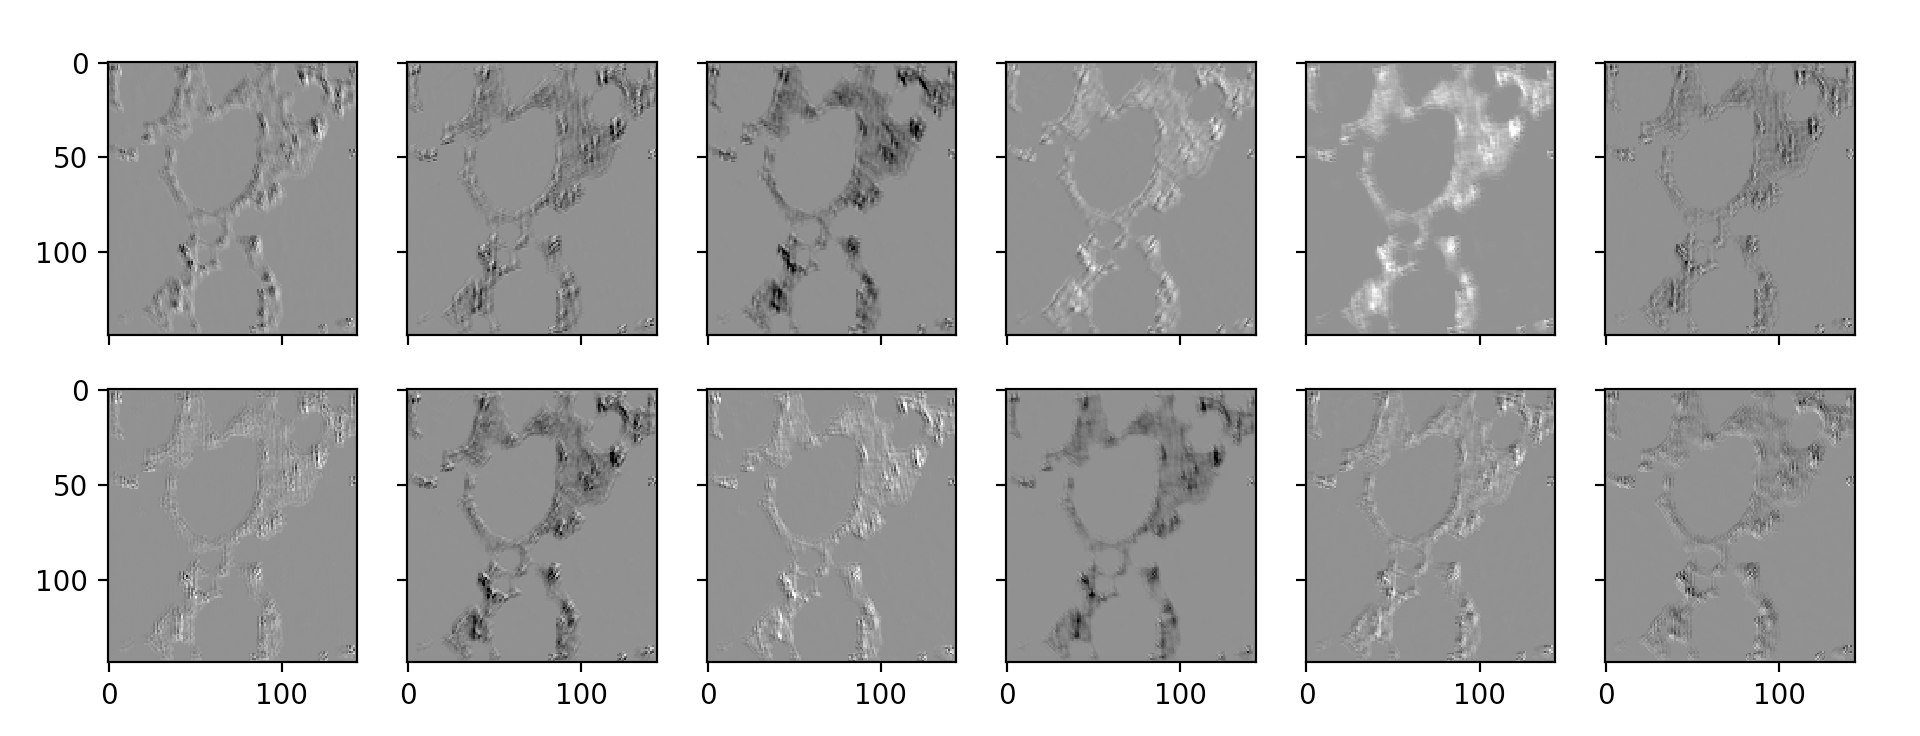
\includegraphics[width=0.75\textwidth]{chapters/hera_ml/figures/classifier-kernels.png}
\caption[An input image propagated through the trained kernels of the first layer of the classifier.]{An input image propagated through the trained kernels of the first layer of the classifier. In this case, the color scale is arbitrary -- contrasts within an image are more important. The axes are labelled by pixel index. Small, high-temperature regions are frequently emphasized.}
\label{fig:CNN_kernel_images}
\end{figure}

\section{Regressing upon reionization parameters}

Cosmological studies often want to go beyond binary classifications, instead seeking to understand the value of some collection of variables that describe physical processes in the Universe. 
The {\sc 21cmfast} \citep{Mesinger.11} and {\sc 21cmmc} \citep{Greig.15} software packages, widely used for realizations of the 21\,cm brightness temperature field, parametrize reionization according to a few variables: the mean free path of ionizing photons (R$_{\rm mfp}$) the minimum virial temperature of star-forming haloes ($T_{\rm vir}$) and the ionizing efficiency of high-redshift galaxies ($\zeta$). 

We investigated the effectiveness of using CNNs to regress upon $\zeta$, holding all other parameters constant. $\zeta$ is defined as:

\begin{equation}
\zeta =  \frac{f_{\rm esc} f_* N_{\gamma}}{1+n_{\rm rec}},
\end{equation}
where $f_{\rm esc}$ is the fraction of ionizing photons that escape into the IGM, $f_*$ is the fraction of galactic gas in stars, $N_{\gamma}$ is the number if ionizing photons produced per baryon in stars, and $n_{\rm rec}$ is the expected number of recombinations per hydrogen atom. The theoretical values of $f_{\rm esc}$ and $f_*$ are highly uncertain at high redshifts \citep[e.g.][]{Paardekooper.15, Meiksin.17}. For the Population II stars at the redshift range of the EoR, $N_{\gamma}\approx4000$ \citep{Barkana.05}. During the EoR, it is expected that $n_{\rm rec}\sim 1$ \citep[e.g.][]{McQuinn.11, Sobacchi.14}. In {\sc 21cmfast}, $\zeta$ is typically varied between 5 and 100, corresponding to $f_{\rm esc}$ values between 5\% and 100\%.

The $\zeta$ is an attractive parameter for an initial analysis, as it has a large effect on the topology of the temperature field and a relatively intuitive interpretation. We generated 2000 21\,cm brightness temperature fields with values of $\zeta$ between 10 and 50, all at redshift $z=10$, in a 150 Mpc box with 200 pixels on a side. Figure~\ref{fig:zeta-30-50} shows two of these fields on the same mK color scale -- one with $\zeta=30$, the other with $\zeta=50$. The effect of increased efficiency is extreme.

\begin{figure}
\centering
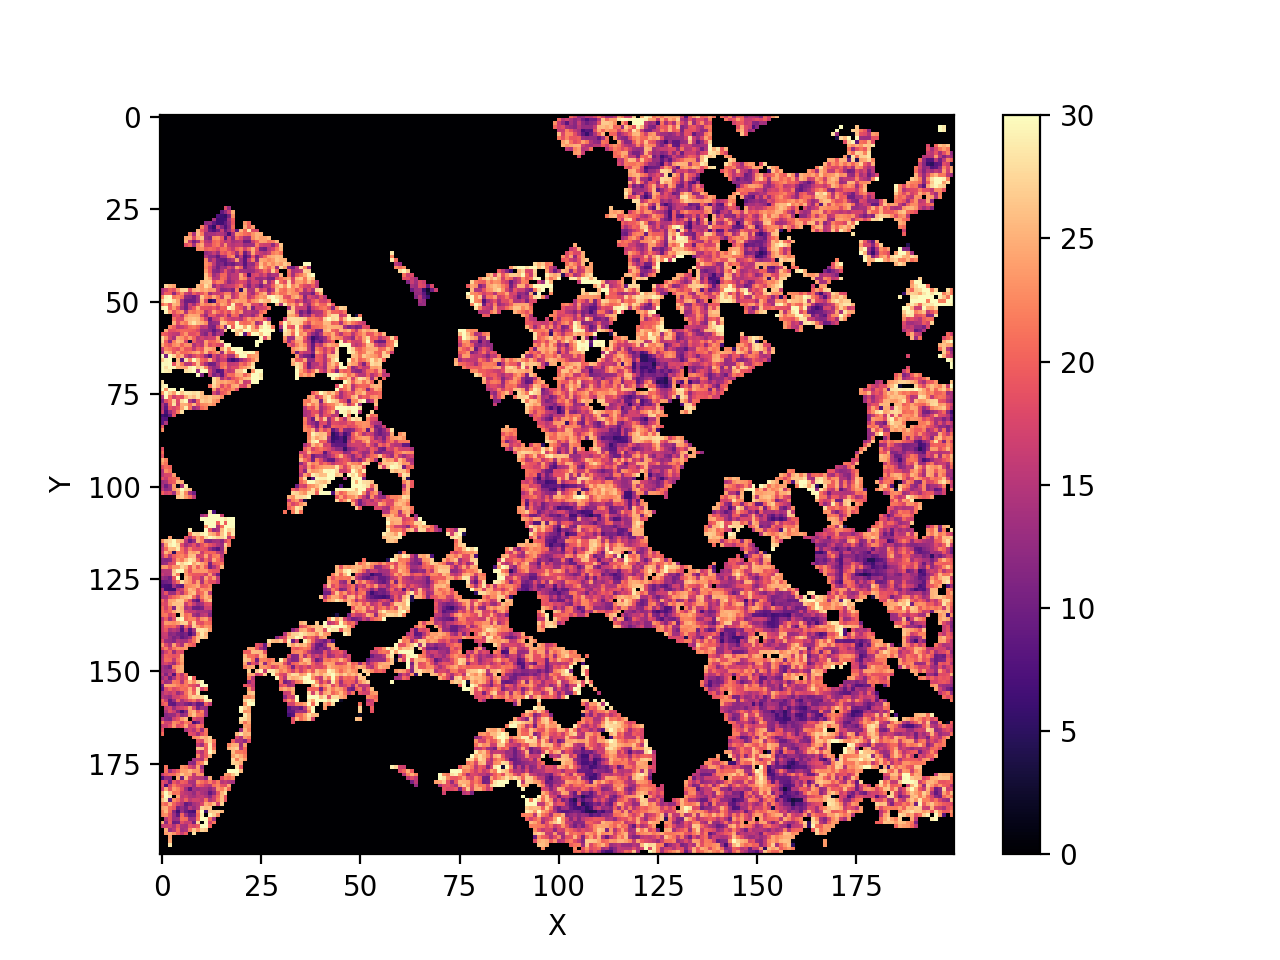
\includegraphics[width=0.49\textwidth]{chapters/hera_ml/figures/zeta30.png}
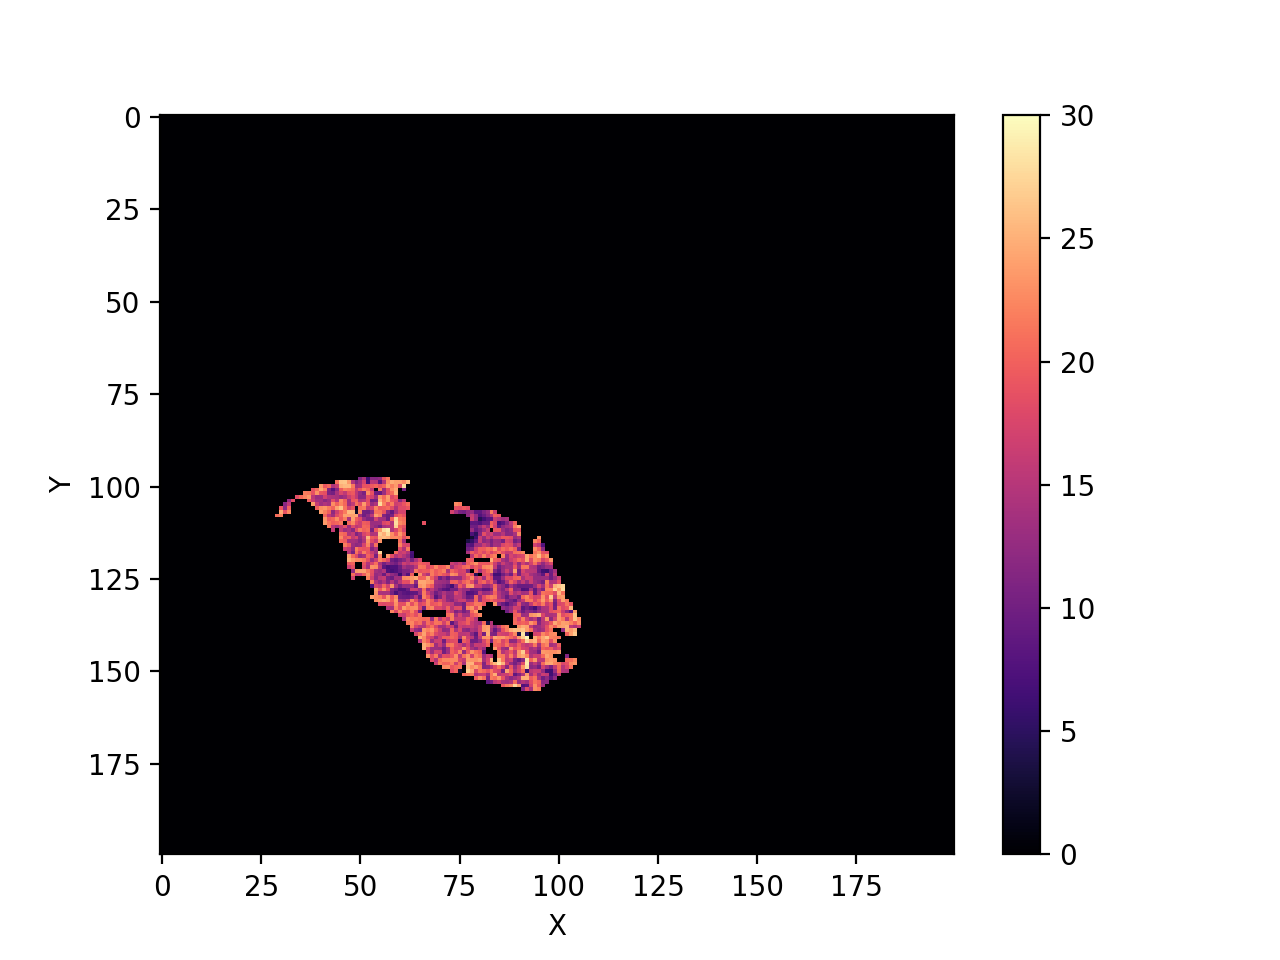
\includegraphics[width=0.49\textwidth]{chapters/hera_ml/figures/zeta50.png}
\caption[The effect of changing $\zeta$ on the 21\,cm brightness temperature field.]{The effect of changing $\zeta$ on the 21\,cm brightness temperature field. The left panel shows a realization of reionization at $z=10$ with $\zeta=30$. On the right, with all other parameters fixed and at the same redshift, is a realization with $\zeta=50$. In the latter, almost the entire region as been reionized. The color scale is in mK.}
\label{fig:zeta-30-50}
\end{figure}

We built a CNN using {\tt keras} \citep{keras} to learn to regress on the value of $\zeta$ for a training set of 1400 images (70\% of the data). We used 3 convolutional layers interleaved with 3 average pooling layers and two dense layers with 10\% dropout. Every kernel and dense-layer weight had an additive linear bias term which could also be learned by the network. We used ReLU activation functions throughout, and a mean squared error cost function. A diagram of the CNN is shown in Figure~\ref{fig:my-cnn}.

\begin{figure}
\centering
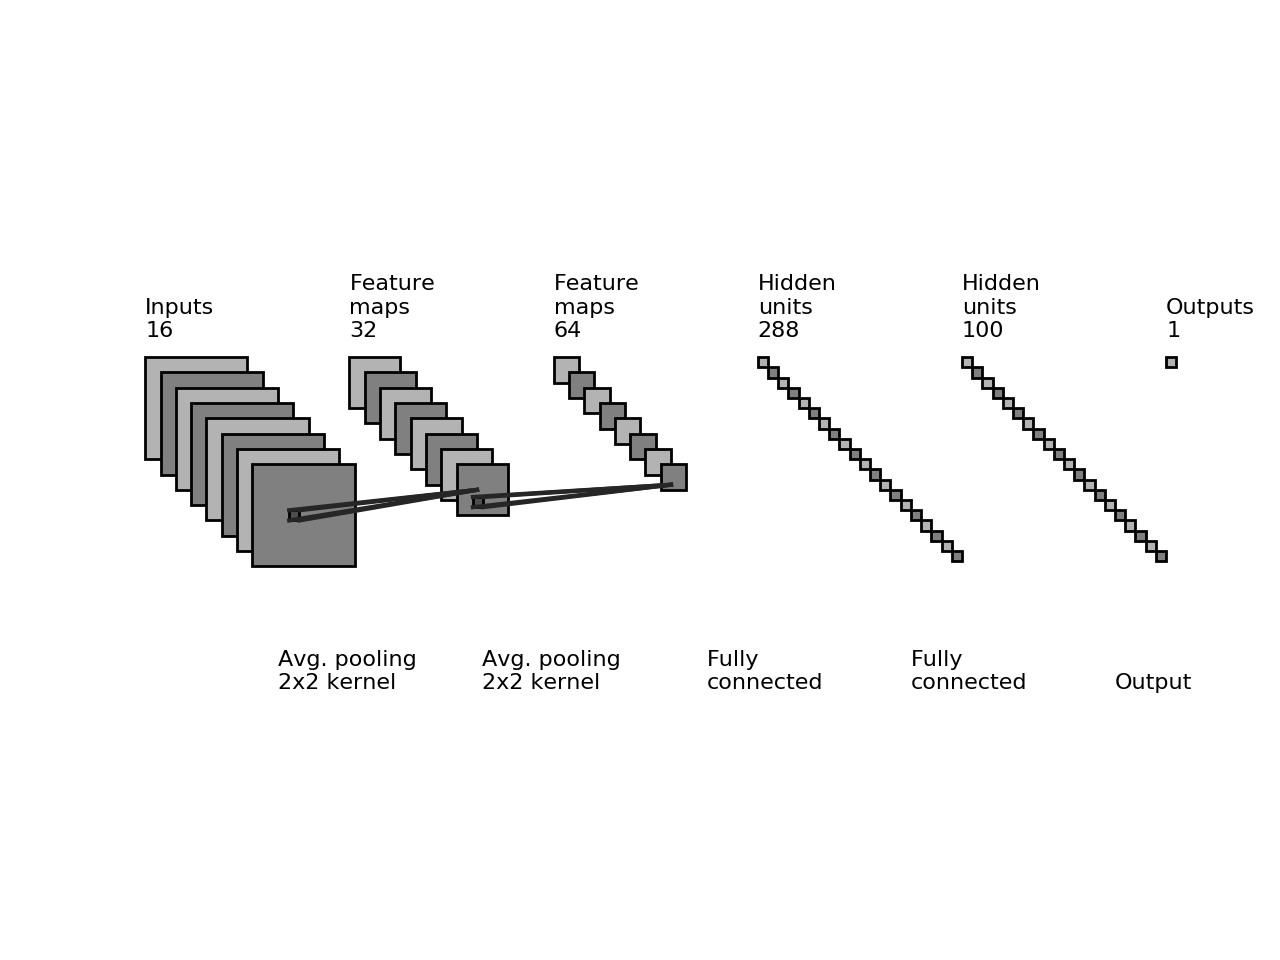
\includegraphics[width=0.8\textwidth]{chapters/hera_ml/figures/my-cnn.png}
\caption{The CNN used for regression.}
\label{fig:my-cnn}
\end{figure}

The results of training are shown in Figure~\ref{fig:CNN_training_results}. For each step of training, we computed the cost function and the coefficient of determination ($R^2$), which measured what fraction of the variance of the overall distribution of $\zeta$ values the model, represented by forward propagation through the CNN, is capturing \citep[e.g.][]{Glantz.90}. The CNN quickly learns to regress to a mean squared error of $\sim 5$, which explains $\sim 80\%$ of the variance of the $\zeta$ distribution. Note that the number of steps is far fewer than the number of images in the training set. This is because, for computational efficiency, we only implemented backpropagation after a batch of training images had propagated forward through the network (this is known as `batch learning'). Batches were chosen randomly from the training set.

\begin{figure}
\centering
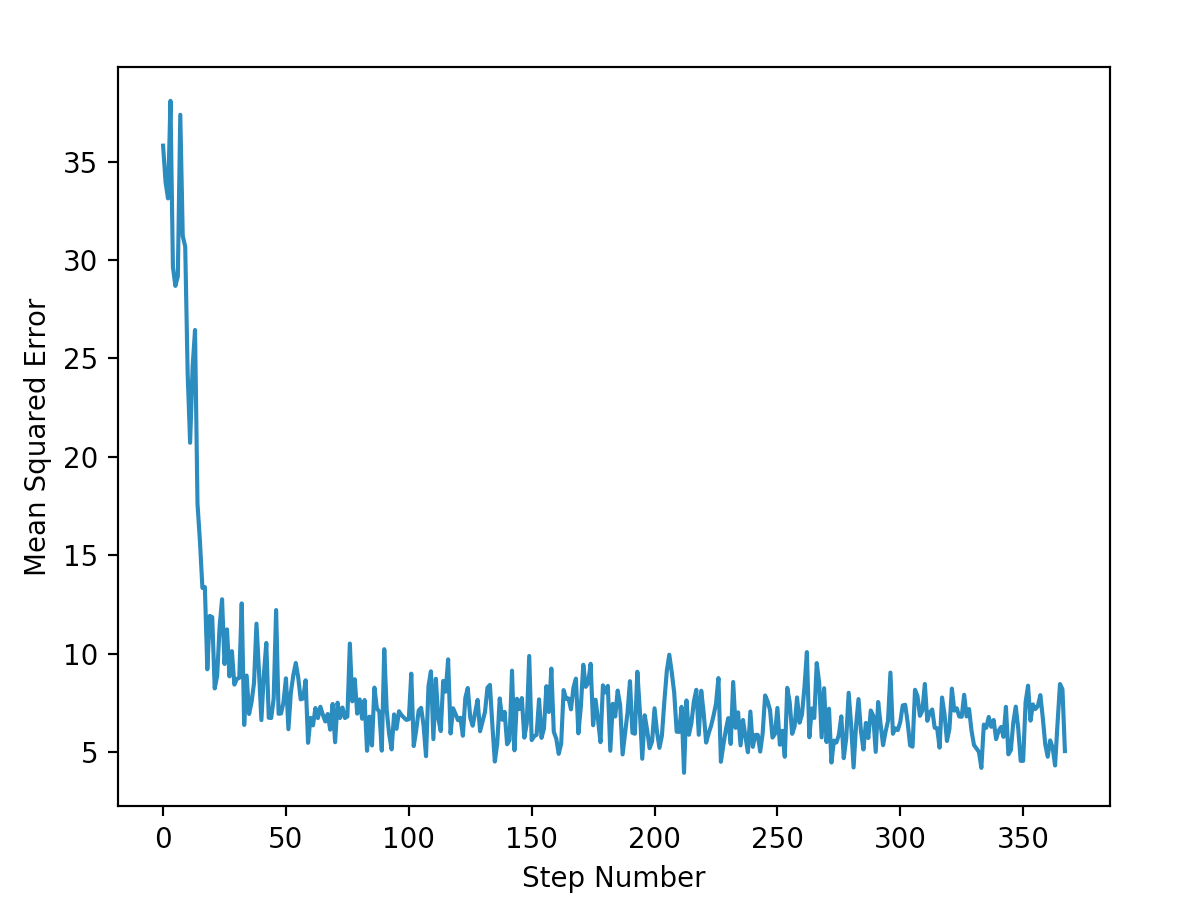
\includegraphics[width=0.49\textwidth]{chapters/hera_ml/figures/zeta-MSE.png}
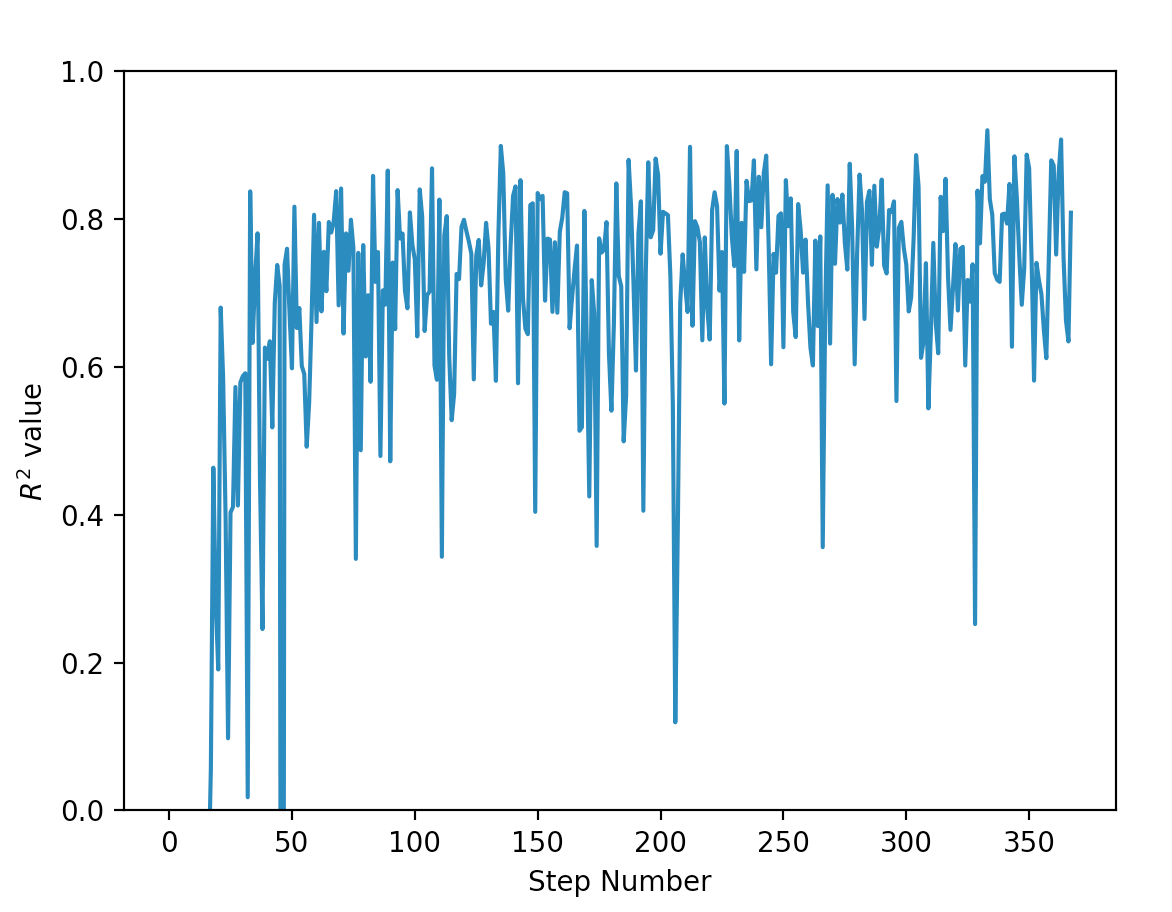
\includegraphics[width=0.49\textwidth]{chapters/hera_ml/figures/zeta-R2.png}
\caption[The results of training the CNN regressor.]{The results of training the CNN regressor. The left panel shows the value of the cost function at each step of training, which quickly reduces to a value of $\sim 5$. At each training step we also calculate the $R^2$ value. Its value suggests that the CNN is capturing about 80\% of the variance of the $\zeta$ distribution.}
\label{fig:CNN_training_results}
\end{figure}

Figure~\ref{fig:compare-zeta} shows the predicted and true values of $\zeta$ from the test set. The CNN was able to predict values to an accuracy suggested by the training results shown in Figure~\ref{fig:CNN_training_results}, but with a systematic bias bias towards lower $\zeta$. Agreement is better at the lowest values of $\zeta$. This is most likely due to the fact that the ReLU function is only extracting positive-valued information. In higher $\zeta$ regimes, as shown in Figure~\ref{fig:zeta-30-50}, reionization occurs very quickly, leaving much of the map reionized and blank -- as far as the CNN can tell, featureless -- so the examples it is able to learn had a lower-valued $\zeta$ than they should. Moving to a `Leaky ReLU' activation function in future attempts would go a ways toward rectifying this issue.

\begin{figure}
\centering
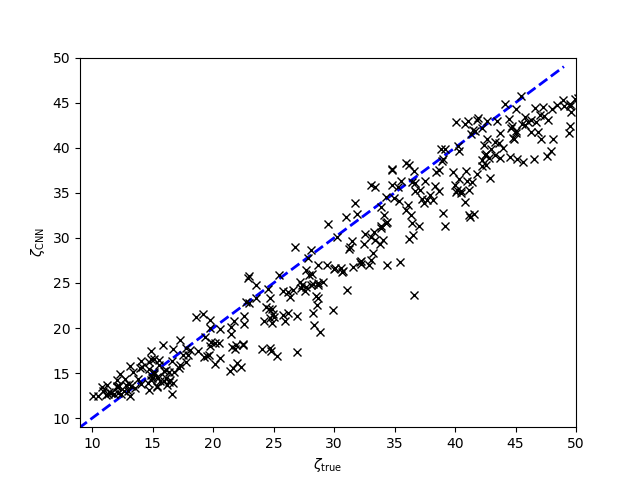
\includegraphics[width=0.8\textwidth]{chapters/hera_ml/figures/CompareZeta.png}
\caption[True vs. predicted values of $\zeta$ from the test set.]{True vs. predicted values of $\zeta$ from the test set. A 1:1 line is overplotted in blue.}
\label{fig:compare-zeta}
\end{figure}

\section{Future directions}

We have presented some basic test that showed that deep learning techniques may be worth developing to analyze 21\,cm measurements. There are a host of directions to pursue in the future, as the field of deep learning is ripe for exploration. An immediate step to take is the development of a formalism for analyzing the trained convolutional kernels. These may contain useful data about what features in a 21\,cm map are the most important for extracting physical parameters. 

By moving to 3-dimensional cosmological maps and kernels, rather than reducing the information to a power spectrum, CNNs should be sensitive to the particular kinds of non-Gaussianity present in the data, without a priori knowledge. The result should be both more precise parameter estimates, due to extracting more information than the traditional methods. We hope to pursue the extraction of the bispectrum of the 21\,cm field, or some proxy for it, in future work.
Related to Chapter~\ref{chapter:ksz_21cm}, one could also build a correlational neural network \citep{Chandar.15} capable of calculating the optimal combination of two fields (for example, the {\sc hi} and dark matter density fields, or the {\sc hi} and kSZ fields) to extract the maximum amount of information \citep{Feng.04}. This may be the most useful avenue to pursue, to build the best tools for combining future survey data. However, it may be difficult to form a training set for such a network.

Finally, Chapter~\ref{chapter:data_prep_and_proc} presented large amounts of work building metrics to understand how to assure the quality of visibility data. The result of that work could be configured into a very large training set of `how and where interferometric visibilities can be corrupted'. The major challenge of using visibility data is their complex nature. Backpropagation of complex-valued input is a contemporary challenge \citep{Guberman.16, Popa.17complex, Zhang.17complex} that is not fully-supported by any mainstream deep learning software packages. However, the volume of data generated by an interferometer such as HERA and the automatic flagging algorithms we have created could prove to be a powerful combination for future deep learning studies.